\documentclass[12pt]{article}

\usepackage{amsmath}
\usepackage{chemfig}
\usepackage{mhchem}
\usepackage[utf 8]{inputenc}
\usepackage{fancyhdr}
\usepackage{pdfpages}
\usepackage{graphicx}

\pagestyle{fancy}
\fancyhead[L]{Jeppe Møldrup}
\fancyhead[C]{Kemi 13}
\fancyhead[R]{18/03-2019}

\begin{document}

\title{Kemi Aflevering 13}
\author{Jeppe Møldrup}
\date{}

\maketitle{}

Alt data fundet i Databogen 07

\section*{Opgave 1}

\begin{enumerate}
        \item[a.] Beregn den formelle stofmængdekoncentration af lorcaserin i den mættede vandige opløsning

                Lorcaserin har den molare masse 195.688 g/mol (Fundet på nettet). Så jeg tager massen og dividerer
                med den molare masse for at finde stofmængden.
                $$n(Lorcaserin)=\frac{0.0709 \ g}{195.688 \ g/mol} = 3.62 \ mmol$$
                Her er det for 1 liter af opløsningen så derfor er den formelle koncentration af Lorcaserin 3.62 mM

        \item[b.] Beregn pH i opløsningen af lorcaserin ved $25^{\circ}$C.

                pKs for lorcaserin er 9.98 (Fundet på nettet).\\
                Så jeg skal bruge formlen for svage syrer i vand (dvs. en pKs på over 4) som lyder
                $$pH = \frac{1}{2}(pK_s-\log{c_s})$$
                Så jeg indsætter værdierne
                $$pH = \frac{1}{2}(9.98-\log{3.62 \ mM}) = 6.71$$
                Så pH for opløsningen er 6.71

        \item[c.] Gør rede for, at omsætningen af lorcaserin i rottehjerner er af 1. orden med hensyn til lorcaserin,
                efter at den maksimale koncentration er opnået.\\
                Bestem halveringstiden for lorcaserin i rottehjerner.

\end{enumerate}
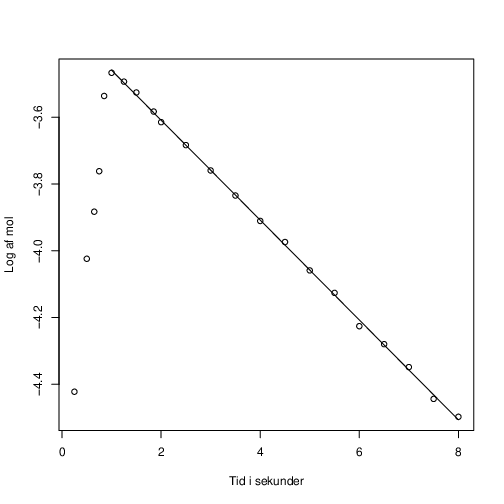
\includegraphics{c.png}
\begin{enumerate}
        \item[] Jeg opstiller et plot med tiden som x og logaritmen af stofmængden som y. Jeg ignorerer så de 5 første punkter da det bare er tiden det tager dem
                at sprøjten midlet ind, og kører lineær regression på resten. Hvis det er en lige linje betyder det at reaktionen er en reaktion af 1. orden.
                Og det ser meget fornuftigt ud.

                Hældningen som er hastighedskonstanten er k=-0.1496.
                Jeg bruger så formlen
                $$T_{1/2} = \frac{log{0.5}}{k}$$
                Så jeg indsætter værdierne
                $$T_{1/2} = \frac{log{0.5}}{-0.1496} = 2.01$$
                Så for hver 2 timer bliver koncentration af lorcaserin halveret

        \item[d.] Tegn en graf, som viser logD for lorcaserin som funktion af pH i vandfasen, og bestem D for lorcaserin ved
                blodets pH 7.4 ved $25^{\circ}$C.\\
                Forklar grafen forløb ud fra lorcaserinmolekylets struktur og stoffets syre-base-egenskaber.

\end{enumerate}
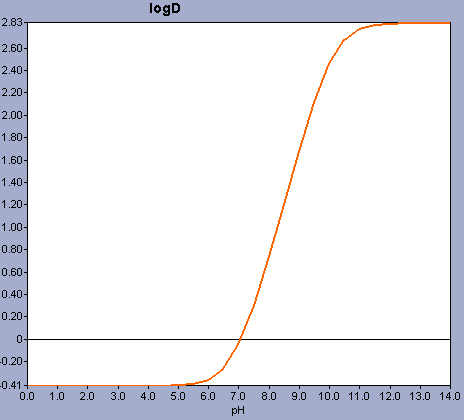
\includegraphics{logd.png}
\begin{enumerate}
        \item[] logD til pH 7.4 er 0.22.\\
                Jo højere en Ph jo mere opløselig er lorcaserin i octan-1-ol. Idet jo mere basisk en opløsning det er, jo flere af
                molekylerne har H+ til at sidde på nitrogen og dermed gør dem mindre polære. Mens jo syrligere det er, jo flere af
                dem har smidt H+'et væk hvilket resulterer i et mere polært molekyle.
\end{enumerate}

\section*{Opgave 2}

\begin{enumerate}
        \item[a.] Angiv, hvilke ioner cobaltforbindelsen indeholder.

                $$\ce{Co^{2+} + Cl_2^-}$$

        \item[b.] Beregn stofmængdekoncentration af B i den fortyndede opløsning

                Under fortyndingen kommer der 20 ml af stamopløsningen i en beholder og fyldt på med propan-2-ol til 50 ml,
                dvs. koncentrationen ganges med 2 og divideres med 5.
                $$\frac{0.0115 \ M \cdot 2}{5} = 0.0046 \ M$$
                Så koncentrationen af B i den fortyndede opløsning er 0.0046 M
\end{enumerate}

\end{document}
